\pdfoutput=1
\pdfcompresslevel=9
\pdfinfo
{
    /Author (Autor)
    /Title (Tytul)
    /Subject (Tematyka)
    /Keywords (Slowa kluczowe)
}
%\documentclass[a4paper,polish,onecolumn,oneside,floatssmall,11pt,titleauthor,wide,openright]{mwrep}
%\usepackage[scale={0.7,0.8},paper=a4paper,twoside]{geometry}
\documentclass[a4paper,onecolumn,oneside,11pt,wide,floatssmall]{mwrep}
% \usepackage{polish}
\usepackage{amsmath}
\usepackage{amsfonts}
\usepackage{amssymb}
\usepackage{amsthm}
\usepackage{bookman}

\usepackage{geometry}
\usepackage[utf8x]{inputenc}
\usepackage[T1]{fontenc}
% \usepackage{t1enc}
% \usepackage[pdftex, bookmarks]{hyperref}
\usepackage[pdftex, bookmarks=false]{hyperref}
\def\url#1{{ \tt #1}}

\usepackage{listings}

% marginesy
\textwidth\paperwidth
\advance\textwidth -55mm
\oddsidemargin-0.9in
\advance\oddsidemargin 33mm
\evensidemargin-0.9in
\advance\evensidemargin 33mm
\topmargin -1in
\advance\topmargin 25mm
\setlength\textheight{48\baselineskip}
\addtolength\textheight{\topskip}
\marginparwidth15mm

\clubpenalty=10000 % to kara za sierotki
\widowpenalty=10000 % nie pozostawia wdów
\brokenpenalty=10000 % nie dzieli wyrazów pomiędzy stronami
\sloppy

\tolerance4500
\pretolerance250
\hfuzz=1.5pt
\hbadness1450

% ŻYWA PAGINA
\renewcommand{\chaptermark}[1]{\markboth{\scshape\small\bfseries \
#1}{\small\bfseries \ #1}}
\renewcommand{\sectionmark}[1]{\markboth{\scshape\small\bfseries\thesection.\
#1}{\small\bfseries\thesection.\ #1}}
\newcommand{\headrulewidth}{0.5pt}
\newcommand{\footrulewidth}{0.pt}
\pagestyle{uheadings}

\usepackage[pdftex]{color,graphicx}
\usepackage[polish]{babel}

% \textheight232mm
% \setlength{\textwidth}{\textwidth}
% \setlength{\oddsidemargin}{\evensidemargin}
% \setlength{\evensidemargin}{0.3cm}
\usepackage[sort, compress]{cite}

%\usepackage{multibib}
%\newcites{bk,st,doc,web}{Książki i~artykuły,Standardy i~zalecenia,Dokumentacja produktów,Publikacje i~serwisy internetowe}

\theoremstyle{definition}
\newtheorem{defn}{Definicja}[section]
\newtheorem{conj}{Teza}[section]
\newtheorem{conjmain}{Teza}
\newtheorem{exmp}{Przykład}[section]

\theoremstyle{plain}% default
\newtheorem{thm}{Twierdzenie}[section]
\newtheorem{lem}[thm]{Lemat}
\newtheorem{prop}[thm]{Hipoteza}
\newtheorem*{cor}{Wniosek}

\theoremstyle{remark}
\newtheorem*{rem}{Uwaga}
\newtheorem*{note}{Uwaga}
\newtheorem{case}{Przypadek}

\definecolor{ListingBackground}{rgb}{0.95,0.95,0.95}

\begin{document}

% kody źródłowe wplatane w tekst
\lstdefinestyle{incode}
{
basicstyle={\footnotesize},
keywordstyle={\bf\footnotesize\color{blue}},
commentstyle={\em\footnotesize\color{magenta}},
numbers=left,
stepnumber=5,
firstnumber=1,
numberfirstline=true,
numberblanklines=true,
numberstyle={\sf\tiny},
numbersep=10pt,
tabsize=2,
xleftmargin=17pt,
framexleftmargin=3pt,
framexbottommargin=2pt,
framextopmargin=2pt,
framexrightmargin=0pt,
showstringspaces=true,
backgroundcolor={\color{ListingBackground}},
extendedchars=true,
% title=\lstname,
captionpos=b,
% abovecaptionskip=1pt,
% belowcaptionskip=1pt,
frame=tb,
framerule=0pt,
}

% kody źródłowe z podpisem
\lstdefinestyle{outcode}
{
basicstyle={\footnotesize},
keywordstyle={\bf\footnotesize\color{blue}},
commentstyle={\em\footnotesize\color{magenta}},
numbers=left,
stepnumber=5,
firstnumber=1,
numberfirstline=true,
numberblanklines=true,
numberstyle={\sf\tiny},
numbersep=10pt,
tabsize=2,
xleftmargin=17pt,
framexleftmargin=3pt,
framexbottommargin=2pt,
framextopmargin=2pt,
framexrightmargin=0pt,
showstringspaces=true,
backgroundcolor={\color{ListingBackground}},
extendedchars=true,
% title=\lstname,
captionpos=b,
% abovecaptionskip=1pt,
% belowcaptionskip=1pt,
frame=tb,
framerule=0.1pt,
}

\renewcommand*\lstlistingname{Wydruk}
\renewcommand*\lstlistlistingname{Spis wydruków}

\pagenumbering{roman}
\renewcommand{\baselinestretch}{1.0}
\raggedbottom

\begin{titlepage}
    % Strona tytułowa
    \vbox to\textheight{\hyphenpenalty=10000
    \begin{center}
	\begin{tabular}{p{107mm} p{9cm}}
	    \begin{minipage}{9cm}
	      \begin{center}
	      Politechnika Warszawska \\
	      Wydział Elektroniki i~Technik Informacyjnych \\
	      Instytut Informatyki
	      \end{center}
	    \end{minipage}
	    &
	    \begin{minipage}{8cm}
	    \begin{flushleft}
	     \footnotesize
	      Rok akademicki 200X/200Y
	    \vspace*{2.75\baselineskip}
	    \end{flushleft}
	    \end{minipage} \\
	\end{tabular}
	\vspace*{3.75\baselineskip}
	\par\vspace{\smallskipamount}
	\vspace*{2\baselineskip}{\LARGE Praca dyplomowa magisterska\par}
	\vspace{3\baselineskip}{\LARGE\strut Imię i Nazwisko\par}
	\vspace*{2\baselineskip}{\huge\bfseries Tytuł pracy\par}

	\vspace*{7\baselineskip}
	\hfill\mbox{}\par\vspace*{\baselineskip}\noindent
	\begin{tabular}[b]{@{}p{3cm}@{\ }l@{}}
	    {\large\hfill } & {\large }
	\end{tabular}
	\hfill
	\begin{tabular}[b]{@{}l@{}}
	Opiekun pracy: \\[\smallskipamount]
	{\large Tytuł Imię i Nazwisko}
	\end{tabular}\par
	\vspace*{4\baselineskip}
    \begin{tabular}{p{\textwidth}}
    \begin{flushleft}
	\begin{minipage}{7cm}
	Ocena \dotfill
	\par\vspace{1.6\baselineskip}
	\dotfill
	\par\noindent
	\centerline{\footnotesize Podpis Przewodniczącego} \par
	\centerline{\footnotesize Komisji Egzaminu Dyplomowego}\par
	\end{minipage}
    \end{flushleft}
    \end{tabular}
    \end{center}}

    % Życiorys
    \newpage\thispagestyle{empty}
    \begin{tabular}{p{5cm} p{12cm}}
    \begin{minipage}{5cm}
    \center
    
\includegraphics[height=6.5cm,width=4.5cm]{../img/foto.jpg}
    \end{minipage}
    &
    \begin{minipage}{12cm}
    \begin{flushleft}
    \par\noindent\vspace{1\baselineskip}
    \begin{tabular}[h]{l l}
    {\normalsize\it Specjalność:} & Informatyka -- \\
    & Inżynieria oprogramowania \\
    & i~systemy informacyjne
    \end{tabular}
    \par\noindent\vspace{1\baselineskip}
    \begin{tabular}[h]{l l}
    {\normalsize\it Data urodzenia:} & {\normalsize 1 stycznia 1980~r.}
    \end{tabular}
    \par\noindent\vspace{1\baselineskip}
    \begin{tabular}[h]{l l}
    {\normalsize\it Data rozpoczęcia studiów:} & {\normalsize 1 października 2002 r.}
    \end{tabular}
    \par\noindent\vspace{1\baselineskip}
    \end{flushleft}
    \end{minipage}
    \end{tabular}
    \vspace*{1\baselineskip}
    \begin{center}
	{\large\bfseries Życiorys}\par\bigskip
    \end{center}

    \indent
    Nazywam się  \ldots.
    \par
    \vspace{2\baselineskip}
    \hfill\parbox{15em}{{\small\dotfill}\\[-.3ex]
    \centerline{\footnotesize podpis studenta}}\par
    \vspace{3\baselineskip}
    \begin{center}
 	{\large\bfseries Egzamin dyplomowy} \par\bigskip\bigskip
    \end{center}
    \par\noindent\vspace{1.5\baselineskip}
    Złożył egzamin dyplomowy w dn. \dotfill
    \par\noindent\vspace{1.5\baselineskip}
    Z wynikiem \dotfill
    \par\noindent\vspace{1.5\baselineskip}
    Ogólny wynik studiów \dotfill
    \par\noindent\vspace{1.5\baselineskip}
    Dodatkowe wnioski i uwagi Komisji \dotfill
    \par\noindent\vspace{1.5\baselineskip}
    \dotfill

    % Streszczenie
    \newpage\thispagestyle{empty}
    \vspace*{2\baselineskip}
    \begin{center}
	{\large\bfseries Streszczenie}\par\bigskip
    \end{center}

    {\itshape
    Praca ta prezentuje \ldots}
    \vspace*{1\baselineskip}

    \noindent{\bf Słowa kluczowe}: {\itshape słowa kluczowe.}
    \par
    \vspace{4\baselineskip}
    \begin{center}
	{\large\bfseries Abstract}\par\bigskip
    \end{center}
    \noindent{\bf Title}: {\itshape Thesis title.}\par
    \vspace*{1\baselineskip}
    {\itshape
    This thesis describes \ldots}
    \vspace*{1\baselineskip}

    \noindent{\bf Key words}: {\itshape key words.}

\end{titlepage}

% ex: set tabstop=4 shiftwidth=4 softtabstop=4 noexpandtab fileformat=unix filetype=tex spelllang=pl,en spell:


\tableofcontents
% \addcontentsline{toc}{chapter}{{Przedmowa1}{vii}}{vii}

% \chapter*{Spis tablic, rysunków i~wydruków}
% \listoftables
% \listoffigures
% \lstlistoflistings

%\setlength{\baselineskip}{7mm}
\newpage
\pagenumbering{arabic}
\setcounter{page}{1}

% \chapter{Wprowadzenie}

Szblon ten jest propozycją składu pracy dyplomowej inżynierskiej lub
magisterskiej. Poniżej znajdują się przykłady pozwalające na
szybkie zapoznanie się z podstawowymi elementami dokumentu takimi jak
tablice, rysunki, wyliczenia itp.

Przed oddaniem tego dokumentu prawidłowo wypełnić jego początkowe strony
tj.:
\begin{itemize}
\item stronę tytułową: rocznik, typ (magisterska/inżynierska),
imię i~nazwisko autora, tytuł, imię i~ nazwisko promotora pracy,
\item życiorys: data urodzenia, datę rozpoczęcia studiów, zdjęcie i~
życiorys autora,
\item streszczenie oraz słowa kluczowe w~języku polskim i~angielskim.
\end{itemize}

Szczegółowe opcje klasy {\tt mwrep}, którą wykorzystuje ten dokument,
opisane są w~dokumentacji.

\section[Tytuł w paginie][Tytuł w spisie treści]{Przykład pierwszy}

Pozostałe pliki (w głównej gałęzi katalogu 5015) reprezentują logikę struktury
PKCS~\#15 oraz certyfikaty (pliki 4545, 4546, 4547). Jej szczegółowy
opis zamieszczono w~\cite[130-140]{bk:ipki}. W~
tablicy \ref{tab:card} zebrano podstawowe dane o~wszystkich plikach.
Rozmiar niektórych plików może być różny dla innych danych wejściowych.
Dotyczy to w~szczególności certyfikatów.

Należy przyjąć, że aplikacja PKCS~\#15 w~karcie zajmuje do 6kB. W~karcie
{\it Cryptoflex 32K} pozsostaje więc około 26 kB możliwych do wykorzystania
przez inne aplikacje. W~szczególności mogą to być kolejne aplikacje PKCS~\#15
o~innym profilu zastosowań.

\begin{table}
\centering
\caption{Wykaz plików karty {\it Cryptoflex 32K} z~aplikacją PKCS~\#15}
\label{tab:card}
\begin{minipage}{.9\textwidth}
\setlength{\baselineskip}{2mm}
\centering
\begin{tabular}{c|c|c|c}
FID\footnote{ang. {\em file identifier} -- identyfikator pliku} & Rozmiar\footnote{rozmiar plików zawierających certyfikaty może być inny (w zależności od umieszczonego certyfikatu)} & Rodzaj pliku & Podstawowe prawa\\
 & (w bajtach) & & dostępu\footnote{stosowane oznaczenia: R~(ang. {\em read}) -- odczyt, U~(ang. {\em update}) -- zmiana, C~-- operacje kryptograficzne, NEV (ang. {\em never}) -- nigdy, CHV1 (ang. {\em cardholder verification}) -- kod uwierzytelniający użytkownika, ALW (ang. {\em always}) -- zawsze, AUT (ang. {\em authenticate}) -- uwierzytelnienie z~użyciem klucza}\\ \hline
3F00		    & --		   & DF\footnote{ang. {\em dedicated file} -- plik dedykoway, katalog}	& -- \\ \hline
0011		    & 27		   & EF\footnote{ang. {\em elementary file} -- plik elementarny}	& R: NEV, U: AUT \\ \hline
0002		    & 8			   & EF, TR\footnote{ang. {\em transparent} -- struktura transparentna, przeźroczysta} & R: ALW, U: NEV \\ \hline
5015		    & --		   & DF		    & -- \\ \hline
4401\footnote{identyfikatory podano bez pełnych ścieżek, zobacz rysunek \ref{ppkcs15fs}}	    & 255		   & EF, TR		    & R: ALW, U: AUT \\ \hline
4402		    & 255		   & EF, TR		    & R: ALW, U: AUT \\ \hline
5031		    & 255		   & EF, TR		    & R: ALW, U: AUT \\ \hline
5032		    & 33		   & EF, TR		    & R: ALW, U: AUT \\ \hline
4545		    & 849		   & EF, TR		    & R: ALW, U: AUT \\ \hline
4546		    & 847		   & EF, TR		    & R: ALW, U: AUT \\ \hline
4547		    & 849		   & EF, TR		    & R: ALW, U: AUT \\ \hline
4946		    & 127		   & EF, TR		    & R: ALW, U: AUT \\ \hline
4B01, 4B02	    & --		   & DF		    & -- \\ \hline
0000		    & 16		   & EF, CHV\footnote{ang. {\em cardholder verification} -- kody służące do uwierzytelnienia użytkownika} & R: NEV, U: CHV1 | AUT \\ \hline
3045, 3047	    & --		   & DF		    & -- \\ \hline
0012		    & 326		   & EF, PRVK\footnote{ang. {\em private key} -- klucz prywatny} & R: NEV, U: AUT, C: CHV1 \\ \hline
1012		    & 330		   & EF, PUBK\footnote{ang. {\em public key} -- klucz publiczny} & R: ALW, U: AUT, C: ALW \\ \hline
2F00		    & 127		   & EF, TR		    & R: ALW, U: AUT \\
\end{tabular}
\end{minipage}
\end{table}

\subsubsection{Założenia}
Dany jest zbiór pewnych maszyn. Każda z~nich charakteryzuje się pewnym
typem i~lokalizacją. Maszyny złożone są z~pewnych modułów.

Każda z~maszyn raportuje do systemu centralnego zdarzenia jakie na niej
zachodzą. Należą one do jednej z~kategorii:
\begin{itemize}
\item normalne zdarzenie
\item błąd -- zdarzenie to zawiera opis zgłaszanego błędu (moduł);
wyróżniamy błędy krytyczne (maszyna nie działa) i~ostrzeżenia (np. brakuje
zasobów dla pewnego modułu)
\item interwencja -- o~kategorii lokalnej (np. maszyna sama się naprawiła)
lub zdalnej (wymagana interwencja człowieka)
\end{itemize}

Na maszynach zachodzą pewne transakcje, których przebieg raportowany jest w~
postaci normalnych zdarzeń (chyba, że w~trakcie pojawi się błąd).

Zdarzenia przechowywane są w~bazie danych. Jest to jedna tabela, w~której
zapisane są dane określające maszynę, data i~czas zdarzenia oraz jego opis.

\subsection{Przykład drugi}

Przykładowa struktura aplikacji zgodnej z~PKCS~\#15 została zaprezentowana
na rysunku \ref{ppkcs15fs}.
Kolejne elementy systemu plików odzwierciedlają instancje obiektów z~danymi
zdefiniowanymi w~PKCS~\#15. Ich szczegółowa budowa, określona z~użyciem
notacji ASN.1 (ang. {\em abstract syntax notation number 1})
przedstawiona jest w~samej normie.

\begin{figure}[htb]
    \begin{center}
	\includegraphics[angle=-90,scale=.6]{img/pkcs15fs.pdf}
	\caption{Przykładowa struktura aplikacji PKCS~\#15}
	\label{ppkcs15fs}
    \end{center}
\end{figure}

\begin{thm}
\label{thm}
Niech $x_1, x_2, x_3, \ldots$ będą dowolnymi zmiennymi o wartościach
należących do zbiorów $X_1, X_2, X_3, \ldots$.
\end{thm}

\begin{note}
Zdanie jest spełnione wyłącznie w dziedzinie $D_1$.
\end{note}

\begin{proof}[Dowód Twierdzenia \ref{thm}.]
Załóżmy, że twierdzenie \ref{thm} nie jest prawdziwe. Wtedy zachodzi:
\begin{equation}
G(t)=L\gamma!\,t^{-\gamma}+t^{-\delta}\eta(t) \qedhere
\end{equation}
\end{proof}

\section{Przykład trzeci}

W~ostatnim dziesięcioleciu, wraz z~silnym rozwojem aplikacji i~urządzeń
wykorzystujących algorytmy kryptograficzne, pojawiło się szereg problemów
związanych z~uniwersalnością zapisu danych wykorzystywanych podczas tych
operacji. Jedna z~amerykańskich firm, będąca liderem na rynku biznesowych
zastosowań kryptografii, postanowiła opracować własne formuły zapisu
informacji kryptograficznych. Brak dyskusji nad proponowanymi zaleceniami
(w przeciwieństwie do głosowania nad normami ISO/IEC) pozwolił na szybkie ogłoszenie
początkowych wersji dokumentów oraz ich wdrożenie. Pomysł przyjął się i~
dzięki temu powstały normy przemysłowe dotyczące kryptografii.

Firma {\bf RSA Data Security, Inc.}, bo o~niej mowa, zaproponowała szereg zaleceń
związanych z~interfejsem dla kryptografii z~kluczem publicznym. Znane są one pod
ogólną nazwą PKCS (ang. {\em Public Key Cryptography Standards}).
Wnioskując jedynie po ogólnym tytule można odnieść wrażenie, że zalecenia
objęły jedynie algorytmy asymetryczne (w których występuje para kluczy -
jawny, zwany publicznym oraz tajny, zwany prywatnym). Twórcy poruszyli
również tematykę związaną z~szerokim zastosowaniem tych algorytmów, dzięki
czemu zalecenia zawierają praktycznie wszystkie najważniejsze i~
najaktualniejsze informacje dotyczące praktycznych zastosowań kryptografii.

Lista dokumentów z~serii PKCS jest następująca:
\begin{itemize}
    \item PKCS \#1: {\em RSA Cryptography Standard} -- zawiera opis
    algorytmu RSA zarówno w~odniesieniu do podpisu cyfrowego jak i~
    kopert cyfrowych\footnote{dokumenty o~identyfikatorach \#2 i~\#4
    zostały połączone w~\#1}
    \item PKCS \#3: {\em Diffie-Hellman Key Agreement Standard} -- opisuje
    sposób implementacji algorytmu uzgadniania kluczy metodą
    Diffiego-Hellmana
    \item PKCS \#5: {\em Password-Based Cryptography Standard} -- zawiera
    opis metody bezpiecznej wymiany kluczy prywatnych
    \item PKCS \#6: {\em Extended-Certificate Syntax Standard} --
    opisuje budowę certyfikatów klucza publicznego X.509
    \item PKCS \#7: {\em Cryptographic Message Syntax Standard} -- jest to
    abstrakcyjny opis danych, które podlegają operacjom kryptograficznym
    \item PKCS \#8: {\em Private-Key Information Syntax Standard} --
    zawiera abstrakcyjny opis dotyczący składowania kluczy prywatnych (w
    formie jawnej i~zaszyfrowanej) wraz z~zestawem atrybutów
    \item PKCS \#9: {\em Selected Attribute Types} -- zawiera definicję
    atrybutów związanych z~certyfikatami, podpisami cyfrowymi i~kluczami
    prywatnymi
    \item PKCS \#10: {\em Certification Request Syntax Standard} --
    opisuje format żądania certyfikacyjnego
    \item PKCS~\#11: {\em Cryptographic Token Interface Standard} --
    opisuje abstrakcyjny interfejs programisty dla różnych typów urządzeń
    kryptograficznych
    \item PKCS \#12: {\em Personal Information Exchange Syntax
    Standard} -- zawiera opis formatu zapisu danych kryptograficznych przez
    aplikacje
    \item PKCS \#13: {\em Elliptic Curve Cryptography Standard} -- zawiera
    opis algorytmów opartych na krzywych eliptycznych
    \item PKCS \#14: {\em Pseudo Random Number Generation} -- zawiera
    opis algorytmów związanych z~generacją liczb
    pseudolosowych\footnote{aktualnie dokument ten jest opracowywany}
    \item PKCS~\#15: {\em Cryptographic Token Information Format
    Standard} -- opisuje sposób zapisu danych w~żetonach kryptograficznych
    (takich jak karty procesorowe)
\end{itemize}

Wszystkie publikacje dostępne są pod adresem internetowym
\url{http://www.rsasecurity.com/rsalabs/}.

\section{Przykład czwarty}

{\it Xfig}\footnote{\url{http://www.xfig.org/}}
i~{\it Dia}\footnote{\url{http://www.gnome.org/projects/dia/},
\url{http://dia-installer.sourceforge.net/}}
to aplikacje wspomagające tworzenie rysunków w~grafice wektorowej.
Pierwsza z~nich przeznaczona jest głownie do tworzenia obrazów
z~prostych elementów takich jak linie, prostokąty, okręgi, łuki.
{\it Dia}, wzorowane na {\it Visio} firmy {\it Microsoft}, posiada
wiele bibliotek graficznych i~jest najbardziej pomocne do
tworzenia skomplikowanych diagramów np. w~UML. Obie aplikacje obsługują
szeroki wachlarz formatów plików graficznych, co pozwala na wykorzystanie
rysunków stworzonych z~ich pomocą w~wielu programach służących do edycji
lub składu dokumentów.

Rysunek \ref{fig:xfig} obrazuje program {\it Xfig} podczas pracy nad jednym
z~rysunków wykorzystanych w~publikacji~\cite{bk:ipki}.
\begin{figure}[htb]
    \begin{center}
    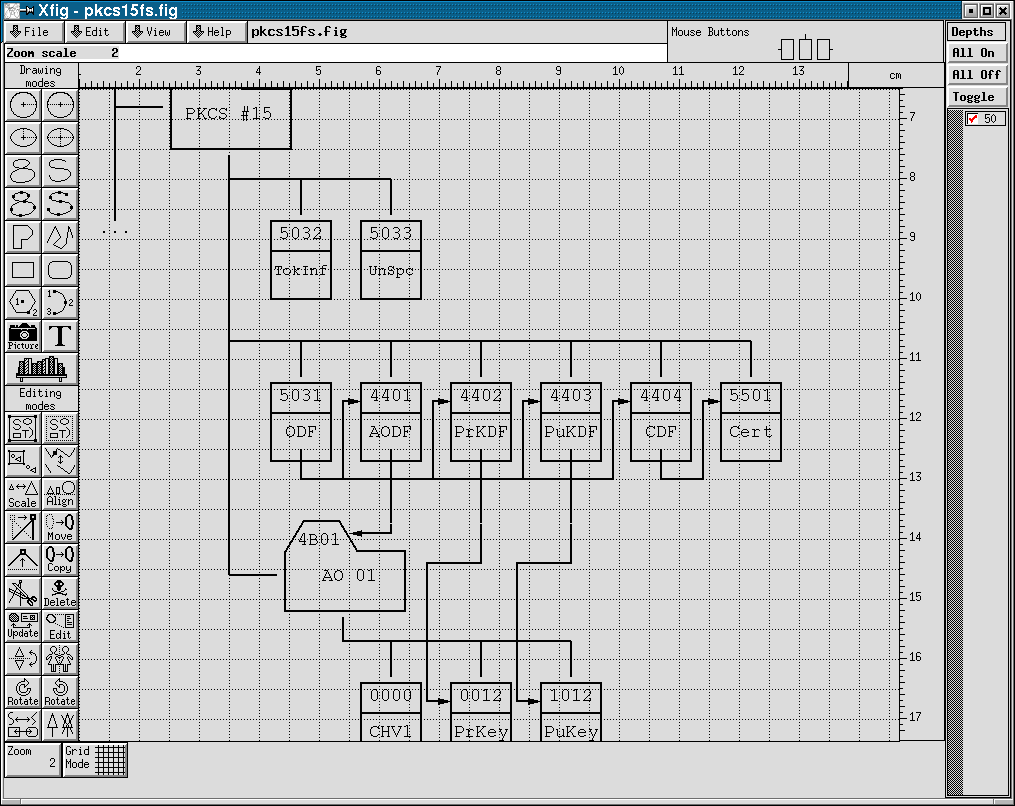
\includegraphics[angle=0,scale=.35]{img/xfig.png}
    \end{center}
    \caption{\em Xfig}
    \label{fig:xfig}
\end{figure}

\section{Przykład piąty}

Po utworzeniu pliku konfiguracyjnego można przystąpić do przygotowania
katalogów służących do przechowywania danych CA (zgodnie z~wcześniej
założonymi nazwami w~{\em openssl.cnf}). Tworzymy katalog {\em ca}, a~w nim
katalogi {\em certs}, {\em crl}, {\em private}, {\em newcerts} oraz pliki
{\em serial.txt} (z wpisem 01) i~{\em index.txt}. Plik {\em openssl.cnf} należy
umieścić na tym samym poziomie co katalog {\em ca}. Oczywiście możliwe jest
zupełnie inne zorganizowanie sposobu przechowywania danych w~CA, jednak
musi ono odpowiadać wcześniej przyjętym założeniom w pliku konfiguracyjnym.

Następnym krokiem przy tworzeniu CA jest wygenerowanie pary kluczy oraz
autocertyfikatu (w przypadku, gdy certyfikat dla centrum nie będzie
poświadczany przez inne centrum certyfikacji) dla centrum certyfikacji.

\begin{verbatim}
# generacja klucza prywatnego RSA o długości 4096 bitów
# do pliku cakey.pem (klucz w formie jawnej)
openssl genrsa -out ca/private/cakey.pem 4096 -config openssl.cnf

# utworzenie autocertyfikatu centrum (cacert.pem) o strukturze
# X.509 i formacie PEM dla klucza jawnego związanego z kluczem
# tajnym cakey.pem
openssl req -new -x509 -days 1825 -key ca/private/cakey.pem -out
    ca/cacert.pem -config openssl.cnf
\end{verbatim}

Po tych operacjach CA jest gotowe do pracy.

\section{Przykład szósty}

Oto przykładowy wydruk:
\begin{lstlisting}[language=Java,style=outcode,caption=Przykładowy wydruk]
import a.b.c;

// komentarz

/*
 * Komentarz...
 */
public class A
{
	int A;
	int B; // zmienna

	A()
	{
		A=1;
		/* to jest komentarz */
	}

	public void metodaA(int i)
	{
		for (int a=i; a<100; ++a)
		{
			short sw=(short)a;
			// ...
		}
	}
}
\end{lstlisting}

A oto wydruk wpleciony w tekst\dots
\begin{lstlisting}[language=C,style=incode]
/* ta funkcja oblicza a+b */
int sum(int a, int b)
{
	int suma=0;

	suma=a+b;

	return suma;
}
\end{lstlisting}
\dots i tekst za kodem.

% \lstinputlisting[language=Java,style=incode]{nazwa pliku}

% ex: set tabstop=4 shiftwidth=4 softtabstop=4 noexpandtab fileformat=unix filetype=tex spelllang=pl,en spell:

%%%% ROZDZIAŁ PIERWSZY %%%%%%%

\chapter{Analiza dziedziny} 
TODO opis tego co znajduje się w tym rozdziale, max 5 zdań


\section{Źródła informacji}

Analiza dziedziny powstała na wskutek agregacji i uporządkowania informacji 
z kilku źródeł. Posłużyłem się literaturą branżową, ustawą i informacjami z 
internetu jak również uzyskałem informację przeprowadzając rozmowy z 
pracownikami hotelu na różnym szczeblu. Miałem okazję rozmawiać z 
recepcjonistką oraz kierownikiem recepcji w dwóch różnych hotelach w 
Warszawie. Poniżej czytelnik znajdzie przefiltrowane, spójne wiadomości z 
branży hotelarskiej.


\section{Historia hotelarstwa} 

Ludzie zmieniali swoje miejsce od tysiącleci. Dlaczego? Powody były różne i 
przez tysiąclecia znacząco się nie zmieniły. Kiedyś wędrówki handlowe, a 
dziś wyjazdy biznesowe. Religijne wyprawy w miejsca kultu, podróże 
turystyczne do atrakcyjnych, bądź historycznych miejsc.     Historia 
hotelarstwa ma bogatą przeszłość i sięga aż II tysiąclecia p.n.e gdzie na 
terenach Bliskiego Wschodu znaleziono pierwsze ślady budownictwa 
nastawionego na gościnę podróżnych. Najstarsze domy zajezdne odnotowano 
wzdłuż szlaków handlowych w miejscach obfitujących w wodę pitną. W 
starożytnej Grecji i Rzymie budowano zajady w miejscach kultu religijnego, 
bądź miejsc odbywania się igrzysk. W czasach Średniowiecza gościny udzielano 
w klasztorach, początkowo nieodpłatnie, z czasem jednak gościna przyjęła 
formę rynkową. Edykt Karola Wielkiego nałożył na klasztory i kościoły 
obowiązek utrzymania hospicjów, gdzie podróżnym udzielano wyżywienia, 
kąpieli i opieki medycznej. Najgęstsza sieć hospicjów znajdowała się na 
terenie dzisiejszej Szwajcarii. Szwajcaria posiada najdłuższe tradycje 
hotelarskie i jest uważana za wzór hotelarstwa takiego jak znamy dzisiaj.


\section{Hotelarstwo i usługa hotelarska}

\subsection{Czym charakteryzuje się hotelarstwo?}

Hotelarstwo to forma działalności gospodarczej charakteryzująca się:
\begin{itemize} 
  \item szczególnym rodzajem gościnności - gościnność za odpłatnością,
  \item na działalność hotelu składają się różnego rodzaju usługi. Główne z 
  nich to usługi bytowe takie jak zapewnienie noclegu oraz wyżywienia,
  \item pobyt gości w hotelach jest z reguły określony w czasie i 
  krótkotrwały,
  \item zakres usług świadczonych przez hotelarzy powiększa się i integruje 
  z innymi działalnościami turystycznymi i rozrywkowymi.
\end{itemize}

\subsection{Definicja usługi hotelarskiej}

Czym jest usługa hotelarska? Na to pytanie odpowie treść ustawy o usługach 
turystycznych \cite{ust:tur}.

\begin{defn}{Usługa hotelarska}

krótkotrwałe, ogólnie dostępne wynajmowanie domów, mieszkań, pokoi, miejsc 
noclegowych, a także miejsc na ustawienie namiotów lub przyczep 
samochodowych oraz świadczenie, w obrębie obiektu, usług z tym związanych.

\end{defn}

Usługi hotelarskie zaspokajają więcej potrzeb niż może to wynikać z 
definicji, a są to: wypoczynek, pożywienie, nocleg, higiena, rekreacja, 
rozrywka, zapewnienie bezpieczeństwa, opieka nad zdrowiem, zapewnienie 
wygody, dobrej atmosfery pobytu i inne drobne usługi.

Pewne usługi są regulowane prawnie, poprzez przepisy dotyczące wymagań 
rodzajowych i kategoryzacyjnych. Jednakże abstrahując od przepisów można 
stwierdzić iż w interesie każdego hotelarza jest zapewnienie tak bogatej 
palety usług jak to możliwe, aby wyróżniać się na rynku i przyciągać gości. 
Spełnienie minimum wymaganego prawnie nie jest szczególnie atrakcyjne z 
punktu widzenia gościa. Więcej o usługach dowiemy się wkrótce.

\section{Kategoryzacja hoteli}
Obiekty, które świadczą usługę hotelarską podlegają kategoryzacji określonej 
prawnie\cite{ust:tur}. Wymagania co do wielkości obiektu, jego wyposażenia, 
kwalifikacji personelu, świadczonych usług, ustalone dla rodzaju i 
kategorii, do których obiekt został zaszeregowany pozwalają stosować 
odpowiednie nazewnictwo: 

\begin{itemize}
  \item hotele - obiekty posiadające co najmniej 10 pokoi, w tym większość 
  miejsc w pokojach jedno- i dwuosobowych, świadczące szeroki zakres usług 
  związanych z pobytem klientów;
  \item motele - obiekty położone przy drogach, dysponujące parkingiem, 
  posiadające co najmniej 10 pokoi, w tym większość miejsc w pokojach jedno- 
  i dwuosobowych;
  \item pensjonaty - obiekty posiadające co najmniej 7 pokoi, świadczące dla 
  swoich klientów całodzienne wyżywienie.
\end{itemize}

Ustawa określa także wymagania w stosunku do kempingów, domów wycieczkowych, 
schronisk młodzieżowych, schronisk oraz pól biwakowych. Zainteresowanych 
odsyłam do ustawy.

\section{Podział usług hotelarskich}   

\section{Ważne definicje} 




%%% OLD BELOW %%%%

\section{Branża hotelarska}

\subsection{Wstęp}

Branża hotelarska jest bardzo różnorodna, począwszy od ogromnych sieci
hotelarskich o zasięgu światowym, które obsługują miliony klientów dziennie i zatrudniają
 jeszcze więcej osób przez średniej wielkości hotele, które działają
 samodzielnie, aż po małe, rodzinne biznesy oferujące swoje usługi
 w turystycznych miejscowościach.
 
  Wszystkie mają jedną wspólną cechę,
 świadczą usługi noclegowe dla swoich klientów. Jest to podstawowy element
 działalności hotelarskiej. Cała reszta usług ma sprawiać, aby klient był
 bardziej zadowolony z pobytu, ponieważ to on jest tutaj najważniejszy.
 
  Dochodzimy tutaj do prostego wniosku, że znakomita
 większość spraw związanych z prowadzeniem hotelu jest taka sama jak dla innych
 biznesów i tyczą się ich te same problemy. W innych biznesach, tam gdzie mamy
 zamówienia, tutaj występują rezerwacje, a towar jest pobytem w hotelu. Istnieje
 cały szereg analogii i dopiero na tym poziomie można zobaczyć czym tak naprawdę
 różni się prowadzenie hotelu od chociażby sklepu wysyłkowego.
 
 Istnieje jednak pewna subtelna różnica pomiędzy branżą hotelarską, a innymi
 branżami. Mianowicie w tym segmencie biznesu jesteśmy bardzo, ale to bardzo
 zależni od poziomu zadowolenia klienta i zależy nam na tym, aby poziom ten był
 jak najwyższy. Jeden nieusatysfakcjonowany klient to strata kilkunastu
 innych potencjalnych klientów, którym ów klient odradzi pobyt w naszym hotelu.
 Jest to szczególnie dotkliwe dla tych mniejszych i średnich hoteli, gdzie nie
 można pozwolić sobie na taką stratę.

\subsection{Klasyfikacja}
W pierwszym spojrzeniu na hotel, jego organizację i hotelowych gości można go
zaklasyfikować do jednej z dwóch kategorii:
\begin{itemize}
  \item Turystyczny
  \item Biznesowy 
\end{itemize}

Hotele, które należą do jednego albo drugiego profilu biznesowego różnią się pod
bardzo wieloma aspektami. Najważniejsze z nich to lokalizacja, wystrój
zarówno wewnętrzny jak i zewnętrzny, rodzaj klientów oraz świadczone usługi
w hotelu. Typowe również jest to, że dla hoteli turystycznych weekendy są zazwyczaj
 droższe niż pobyty w środku tygodnia. Sytuacja jest zupełnie odwrotna dla grupy
 biznesowej. Charakterystycznym dla hoteli turystycznych jest to, że obłożenie
 hotelu jest wysokie zazwyczaj tylko w tzw. sezonie turystycznym, a przez resztę
 roku utrzymuje się na niższym poziomie.
 
 W klasie hoteli o profilu biznesowym średnie obłożenie będzie zazwyczaj wyższe
 niż dla tych z grupy turystycznej, ale na pewno nie jest to reguła, która się
  sprawdza zawsze. Tutaj również istnieje sezon, w którym obłożenie hotelu
  osiąga swój szczyt. Pomijając specjalne okoliczności takie jak EURO2012, takim
  sezonem jest sezon konferencyjny, który zaczyna się na przełomie marca i kwietnia.
  
  Dla hoteli z profilu biznesowego następuje 
 jeszcze jeden podział ze względu na politykę wynajmowania albo łóżek albo pokoi.
   
 Wytłumaczenie różnic w politykach:
 
 W jednym hotelu możemy wynająć pokój np.
 3 osobowy i cena pozostanie taka sama jeśli będziemy tam sami albo w dwie osoby albo w pięć jeśli jest to hotel,
  który działa zgodnie z polityką wynajmowania pokoi. Inna sytuacja nastąpi w hotelach, które wynajmują łóżka,
   cena będzie się różniła dość znacznie. Takie hotele również
   zazwyczaj nie godzą się na to aby w pokoju nocowało więcej osób niż liczba łóżek. 
   Hotele klasy turystycznej zazwyczaj prowadzą politykę wynajmowania łóżek, a hotele klasy biznesowej wynajmowania pokoi.

\subsection{Rezerwacja}
Elementem wspólnym dla każdego hotelu jest rezerwacja.
Rezerwacja to dokument, który zapowiada pewne zdarzenie
z przyszłości jakim jest pobyt w hotelu w określonych dniach,
pokoju, warunkach i osobach, które ten pobyt będą odbywać.

Niestety nie ma utartego schematu jednej rezerwacji i tego jakie informacje
powinna zawierać. Można wyszczególnić pewien zbiór informacji, który zawiera się
na każdej rezerwacji, a przynajmniej powinien się zawierać. Jednak istnieją
hotele, które pozwalają na wprowadzanie wielu dodatkowych informacji do
rezerwacji. Zazwyczaj są to hotele wysokiej klasy, a informacje które możemy
podać odnoszą się np. do typu poduszki jaki chcemy, rodzaju łóżka lub innych
upodobań. Więcej informacji o tym co może zawierać informacji znajdziesz w
sekcji \ref{informacje_na_rezerwacji}


\subsubsection{Gwarantowana rezerwacja}
Rezerwacja zazwyczaj wymaga pewnej gwarancji ze strony rezerwującego, ponieważ
hotel zobowiązuje się, aby pokój, na który prowadzona jest rezerwacja
był w danym czasie dostępny. Jeśli kto inny chciałby wtedy dokonać rezerwacji 
zakładając, że był to ostatni wolny pokój to wtedy stracimy klienta jeśli 
rezerwujący się wycofa albo nie przyjdzie. Potrzebny jest zatem pewien  
mechanizm zabezpieczający hotel przez potencjalnymi stratami. 

Typowy mechanizm gwarantowanej rezerwacji dla klientów indywidualnych przy dokonywaniu 
jej online polega na podaniu numeru karty kredytowej, która w przypadku 
nieodwołania rezerwacji przed określonym terminem przez hotel zostanie obciążona pewną karą 
również określoną przez hotel. Dla klientów indywidualnych niektóre hotele 
umożliwiają dokonywanie rezerwacji niegwarantowanej. Polega to na tym, 
że można dokonać rezerwacji z datą przyjazdu na dzisiaj bez podawania 
numeru karty, ale jest ona trzymana do określonej godziny, 
zazwyczaj 16 czasu lokalnego, po której to już nie mamy pewności 
czy pokój nie zostanie wynajęty komuś innemu. Możliwość dokonania
niegwarantowanej rezerwacji jest świadczona tylko przez niektóre hotele.
Zazwyczaj każdy woli być zabezpieczony. 

Niegwarantowana rezerwacja to dość wygodne rozwiązanie szczególnie w krajach jak
Polska, gdzie posiadanie karty kredytowej nie jest jeszcze tak popularne. Warto zaznaczyć, że sposób gwarancji rezerwacji 
nie ma nic wspólnego z metodą płatności za pobyt. Przykładowo gwarantować
rezerwacje można kartą kredytową, a płacić gotówką albo przelewem albo innym
środkiem płatności akceptowanym przez hotel.


\subsubsection{Informacje na rezerwacji}
\label{informacje_na_rezerwacji}
Rezerwacja przechowuje dość sporo informacji. Standardowa porcja informacji, 
które są wymagane aby dokonać rezerwacji jest następująca:
\begin{itemize}
  \item Numer rezerwacji,
  \item data przyjazdu,
  \item data wyjazdu,
  \item rodzaj pokoju,
  \item dane rezerwującego
  \begin{itemize}
    \item imię,
    \item nazwisko, 
    \item adres, 
    \item kontakt jak e-mail, numer telefonu.
  \end{itemize} 
  \item kto płaci
\end{itemize}

Oprócz takich podstawowych informacji bardzo często możemy podać także wiele 
innych informacji. Często umożliwiają to hotele o wysokim standardzie. Niektóre
z możliwych informacji to np. preferencje:
\begin{itemize}
  \item czy pokój dla palących czy niepalących,
  \item umiejscowienie pokoju,
  \begin{itemize}
    \item niskie piętro,
    \item wysokie piętro,
    \item blisko windy,
  \end{itemize}
  \item widok,
  \item rodzaj poduszki.
\end{itemize}

Podać można także takie informacje jak:
\begin{itemize}
  \item kod promocyjny - często hotele biznesowe, a szczególnie duże sieci
  hotelarskie o światowym zasięgu oferują programy lojalnościowe, w których
  zbiera się punkty, które później można wymienić np. na voucher na darmowy
  pobyt w hotelu. Kod promocyjny odnosi się właśnie do tych nagród,
  \item przynależność do grupy,
  \item przynależność do korporacji,
  \item przynależność do agenta biura podróżniczego,
  \item planowana godzina przyjazdu,
  \item informacje dodatkowe dla recepcji jak specjalne życzenia bądź uwagi
\end{itemize}

Inne informacje zależą tylko od inwencji własnej osoby odpowiedzialnej za hotel,
która będzie chciała zrobić tak żeby klienci czuli się jak najlepiej. Część z nich 
taka jak odpowiedni kod grupy lub korporacji ma związek z typem klientów hotelu.
Typ klientów został opisany w sekcji \ref{rodzaje_klientow}

\subsubsection{Sposób dokonywania rezerwacji}
Rezerwacji można dokonywać:
\begin{itemize}
  \item online – uzupełniając formularz na stronie hotelu
  \item telefonicznie – podając dane pracownikowi recepcji. Wtedy przez 
  całą procedurę przeprowadzi nas pracownik recepcji. Wszystkie dane powtarzane
  są dwa razy w celu sprawdzenia ich poprawności przez obie strony.
  \item osobiście – jeśli chcemy dokonać osobiście rezerwacji w hotelu w
  recepcji to możemy to zrobić, po czym dostajemy albo klucz do 
  pokoju – jeśli chcieliśmy mieć pokój na teraz albo potwierdzenie rezerwacji, 
  które jest dokumentem zawierającym podstawowe dane rezerwacji oraz 
  numer rezerwacji
\end{itemize}

\subsubsection{Odwołanie rezerwacji}
Odwołanie rezerwacji jest zazwyczaj możliwe i nie wiąże się z karą jeśli 
rezerwacja zostanie odwołana przed określonym terminem. Zazwyczaj, ponieważ
niektóre hotele całkowicie zabraniają odwoływania rezerwacji zatem zawsze wiąże
się to z utrzymaniem karą. Przykładem są, niektóre hotele w sieci Marriott.
Te hotele, które umożliwiają odwołanie rezerwacji wymuszają pewne
zasady na których to odwołanie się odbywa zazwyczaj jest to określona godzina,
do której możemy odwołać rezerwację. Przykładowy termin to godzina 16 czasu
lokalnego hotelu w planowanym dniu przyjazdu. Może to być także zupełnie inny termin arbitralnie wybrany przez osobę za to odpowiedzialna. 
  Po określonym terminie odwołanie jest możliwe jeśli hotel ma taką politykę. 
  Zazwyczaj odwołanie rezerwacji przeprowadza się telefonicznie dlatego także to w gestii 
  pracownika hotelu jest ustalenie co zrobić, czy odwołać rezerwację bez żadnej kary nawet po terminie
   czy jeśli klient coś kręci to nie dać się nabrać i odpowiednio zareagować. 
  Ważne jest tutaj odpowiednie przeszkolenie pracowników i ich doświadczenie.
  
  Należy pamiętać o tym, że jeśli mówimy, że nie możemy przyjechać w danym dniu,
  ponieważ lot nam się opóźnił to taka informacja jest łatwa do sprawdzenia
  przez pracownika hotelu i jeśli pracownik ma podejrzenie, że coś jest nie tak
  to właśnie zostanie to sprawdzone.

Jeśli nie pojawimy się w hotelu w dniu rezerwacji to typowym mechanizmem jest
to, że w następnym dniu rezerwacje które nie zostały zrealizowane oznaczane są
jako NO SHOW. Dalsza procedura zależy od hotelu albo obarczą karą tego kto
gwarantował rezerwację albo będą próbowali skontaktować się z rezerwującym. Nie
ma tutaj mechanizmu uniwersalnego. Należy jednak pamiętać, że karanie klienta
jest rozwiązaniem, które przynosi korzyści tylko krótkoterminowo, a hotel
powinien być zainteresowany zyskami długoterminowymi dlatego też warto aby
istniała procedura opierająca się na wyjaśnienie przyczyny, dialog z klientem i
wspólne porozumienie.

\subsubsection{Relokacja rezerwacji}
Relokacja rezerwacji polega na przesunięciu w czasie daty 
przyjazdu lub/i wyjazdu. Jest to możliwe do zrobienia. Warto jednak pamiętać o
tym że o ile sama relokacja nic nie kosztuje to cena rezerwacji może 
wzrosnąć, jeśli przesuwamy ją na termin, w którym cena pobytu jest po prostu 
większa. Prosta zasada to nowy termin, nowa wycena. Relokacja jest możliwa 
wtedy gdy mamy wolne pokoje w terminie, na który klient chce przesunąć
rezerwację.

\subsubsection{Stan rezerwacji}
Rezerwacja znajduje się w kilku możliwych stanach. Czytelników wrażliwych na
anglicyzmy zapraszam do następnej sekcji. Osobiście nie podejmuje się tłumaczeń
poszczególnych stanów, a jedynie wyjaśniam co znaczą. Zaletą jest to, że
praktycznie wszędzie na świecie spotkamy te same angielskie nazwy. Pierwsze dwie
stany są trochę bliskie wewnętrznej organizacji systemu, reszta jest już istotna
z punktu widzenia człowieka.

\begin{description}
\item[Request denied] żądanie rezerwacji zostało odrzucone
\item[Requested] żądanie rezerwacji zostało przyjęte, ale pobyt nie został
jeszcze zarezerwowany
\item[Reserved] pobyt został zarezerwowany
\item[Cancelled] rezerwacja została odwołana przez klienta
\item[In-house] klient zameldował się do hotelu. Od tego momentu zaczyna się
pobyt
\item[No-show] klient na którego była rezerwacja nie wmeldował się w dniu
przyjazdu
\item[Checked out] gość hotelowy wymeldował się z hotelu. Koniec pobytu.
\item[Waitlisted] rezerwacja oczekuje na potwierdzenie
\end{description}

Można by jeszcze wskazać jeden stan, a mianowicie stan \emph{Check-in}.
Rezerwacja znajduje się w tym stanie, gdy obecny dzień jest dniem przyjazdu
klienta.

\subsubsection{Typowy przebieg}
Typowy przebieg wygląda następująco. Składamy rezerwację przez internet i ma
wtedy ona stan \emph{Requested}, a wkrótce potem \emph{Reserved}. Następnie
nadchodzi dzień przyjazdu i rezerwacja ma stan \emph{Check-in}. Gdy przyjeżdżamy
do hotelu i zgłaszamy się w recepcji recepcjonista/tka przyjmuje nas, a
rezerwacja zmienia swój stan na \emph{In-house}. Odbywamy pobyt i cieszymy się z
wypoczynku, aż przychodzi dzień wyjazdu. Wymeldowujemy się z hotelu, a
rezerwacja zmienia swój stan na \emph{Checked out}.

\subsection{Rodzaje klientów}
\label{rodzaje_klientow}
Gości hotelowych można podzielić na parę kategorii. Przynależność do danej
kategorii ma wpływ przede wszystkim na cenę pobytu jak również na inne 
dodatkowe usługi oferowane przez hotel. 

Podział wygląda następująco:
\begin{itemize}
  \item klient indywidualny,
  \item klient korporacyjny,
  \item klient grupowy,
  \item klient związany z agentem biura podróżniczego,
  \item klient stały.
\end{itemize}

\subsubsection{Klient indywidualny}
Klient indywidualny jest to po prostu zwykła osoba z ulicy, która zazwyczaj
płaci najwyższą stawkę za pobyt i inne usługi dodatkowe jakie oferuje hotel.

\subsubsection{Klient korporacyjny}
Klient, który należy do korporacji, która ma z hotelem podpisaną umowę.
Zazwyczaj wygląda to tak, że korporacja zobowiązuje się do wykorzystania 
pewnej liczby pobytów w roku co powoduje iż cena jest odpowiednio niższa.
Wszystkie szczegóły reguluje umowa.

\subsubsection{Klient grupowy}
W hotelach czasem organizowane są konferencje, bale bądź wystawy. Uczestnik
takiego wydarzenia należy do grupy.

Zdarza się także, że na czas pobytu grupy w hotelu w recepcji ustawiane 
jest dodatkowe stanowisko, które obsługuje tylko i wyłącznie członków danej 
grupy. Taka sytuacja zazwyczaj ma miejsce w większych hotelach.

Ceny dla takich grupowych klientów, podobnie jak z klientami korporacyjnymi,
reguluje umowa pomiędzy hotelem, a organizatorem danego wydarzenia.

\subsubsection{Klient związany z agentem biura podróżniczego}
Przy wyszukiwaniu miejsca na spędzenie wakacji udajemy się zazwyczaj do biura
podróżniczego, które oferuje nam kompleksowo zaplanowane wakacje.

Między innymi elementami układanki znajduje się hotel, w którym odbędziemy pobyt
i właśnie taki klient jest klasyfikowany do tej grupy.

Również w tym przypadku występuje umowa pomiędzy agencją turystyczną, a hotelem.

\subsubsection{Klient stały}
Istnieją tacy klienci którzy po prostu mieszkają w hotelach. Przykładem może być
Pan Krauze i Hotel Marriott.  

Taki klient ma gwarancje tego, że zawsze dostaną
swój ulubiony pokój więc zazwyczaj jest on dla nich trzymany wolny. Klient stały
ma szereg udogodnień zarówno w usługach jak i płatnościach np. przekładanie
płatności lub łączenie ich za wiele pobytów.

Tutaj istnieje ogromna dowolność w obsługiwaniu takiego klienta i nie należy
tego ograniczać żadnymi ramami.

\subsubsection{Grupy w kontekście rezerwacji}
Członkowie grupy lub klienci korporacyjni mają wszystko albo opłacone 
albo płacą sami za siebie, wtedy jest to cenowo nadal mniej niż dla klientów 
indywidualnych. W przypadku gdy wszystko jest opłacone po prostu
wystawiana jest faktura na odpowiednią firmę, z którą związana jest dana
grupa. Wszystko zależy od tego jak sporządzona zostanie umowa pomiędzy hotelem,
a innym podmiotem gospodarczym.

Każdy uczestnik grupy ma swoją własną rezerwację. To, że należy do grupy jest 
odnotowane w informacjach zawartych w rezerwacji. To samo tyczy się klientów 
należących do innej kategorii. Rezerwacja jest wystawiana na konkretne osoby, 
a nie firmy z którymi podpisana jest umowa.

\subsection{Długość pobytów}
Wiadomym jest, że istnieje dowolność w długości pobytów, choć czasem mogą być
pewne różnice w cenie za noc jeśli spędzimy jedną noc lub trzy pod rząd.

To co jednak nie jest tak bardzo rozpowszechnione to to, że w hotelach,
zazwyczaj w tych z klasy biznesowej, możliwe jest odbycie krótkoterminowego
pobytu.
\subsubsection{Krótkoterminowy pobyt}
Jeśli potrzebujemy się tylko odświeżyć albo spędzić kilka godzin w klientem na
rozmowie albo wystąpił inny realny scenariusz to warto skorzystać z opcji jaką
jest pobyt do godziny po południowej.
Przykładowo możemy wynająć pokój w taki sposób, że musimy go opuścić np. do
godziny 16 i wtedy nie zapłacimy standardowo za noc, tylko odpowiednio mniej.
Nie jest to przelicznik godzinowy. Po prostu można odbyć pobyt do południa i
koszt takiego pobytu będzie na pewno mniejszy niż byśmy wynajęli pokój na noc.

\subsection{Konferencje}
Wydawać by się mogło, że głównym źródłem dochodu dla hotelu jest oferowanie
pokoi. Jednak często jest tak, że spora część dochodu dla hotelu ma źródło z
przyjmowania konferencji. Oczywiście nadal w grę wchodzą pokoje dla uczestników
konferencji, ale sytuacja całościowo wygląda inaczej dlatego warto o niej
wspomnieć.

Są hotele, które utrzymują się praktycznie tylko z organizowania konferencji, a
pobyty dla osób indywidualnych są bardzo małą częścią zysku hotelu. Przykładem
takiego hotelu jest hotel Gromada w Warszawie, który posiada największą bazę sal
konferencyjnych w Warszawie, a przynajmniej jedną z większych.

Jak już wspomniałem o salach konferencyjnych to jest to właśnie nieodzowny
element konferencji. Oprócz tego trzeba ulokować jeszcze uczestników
konferencji w pokojach. Zazwyczaj jest tak, że pokoje dla uczestników
konferencji są obok siebie. Nie jest to reguła.

W niektórych hotelach, na czas konferencji lub innego grupowego wydarzenia
uruchamiane jest specjalne stanowisko w recepcji, które obsługuje tylko
uczestników danej konferencji. Przykładem takiego hotelu może być hotel Marriott
w Warszawie. Wszystko zależy od wielkości grupy i szczegółów umowy jaka jest
podpisana między hotelem, a organizatorem konferencji. Nie mniej jednak
możliwość osobnego stanowiska istnieje. 

Przypomnę jeszcze, że każdy uczestnik konferencji ma własną rezerwację.

\subsection{Usługi}
Usługi, pod tym pojęciem kryje się wiele. Sekcję tą poświęcam na opisanie tych
najczęściej zamawianych oraz nakreślam jakie inne usługi mogą być oferowane
abstrahując od takich jak trufle na złotej tacy podane do łóżka.

\subsubsection{Definicja usługi}
Usługa to pewna korzyść, z której odpłatnie lub nie może skorzystać klient
podczas swojego pobytu. Pod to pojęcie można by podciągnąć bardzo wiele rzeczy.
Przykładowo korzystanie z basenu hotelowego, siłowni lub spa. Chciałbym się
jednak skupić nie na usłudze w sensie bogatej oferty hotelowej, a na tych
usługach, które wymagają specjalnego traktowania przez obsługę hotelu innego niż
dopisania tego do rachunku.
\subsubsection{Przykłady usług}
Przykładem takiej usługi, która może być przydatna dla zwykłego człowieka jest
budzenie. Zamawiamy w recepcji budzenie na godzinę taką i taką i mamy nadzieje,
że zostaniemy o tej godzinie obudzeni. Czy to nastąpi poprzez telefon czy
stukanie do drzwi to już zależy od wewnętrznej organizacji.

Innym przykładem usługi, może być dostarczenie klientowi np. świeżych elementów
wyposażenia łazienkowego takiego jak ręcznik albo kosmetyki. Takie usługi są
zazwyczaj dodatkowo płatne. Oczywiście na stanie dostępne są ręczniki i
podstawowe kosmetyki. Ta usługa natomiast dotyczy dodatkowych przyborów.

Kolejna usługa to np. dostarczenie do pokoju koja oraz kuwety dla naszego
pupila.

Zdarza się również, że za usługę dostępu do internetu trzeba zapłacić. Zatem
zależnie od hotelu można to traktować albo jako usługę dodatkową albo jako
ofertę hotelu wliczoną w cenę.

Nie sposób jest wymienić wszystkich możliwych usług, ponieważ wszystko zależy od
wyobraźni klienta i tego czy obsługa hotelu może i chce sprostać zadaniu. A jak
wiemy powinniśmy robić wszystko, aby zadowolenie klienta było jak największe.
Oczywiście wszystko ma swoją cenę, a cenę za niestandardowe rzeczy ponosi
klient.

\subsubsection{Klasyfikacja usług}
Można by zatem spróbować sklasyfikować usługi biorąc pod uwagę to czy system
informatyczny może pomóc w ich zrealizowaniu czy też nie. Czynnika ludzkiego
nie sposób jest wyeliminować w spełnianiu zachcianek klienta, tak więc tutaj
odgrywa on rolę szczególną.

System na pewno może pomóc w zapamiętaniu kto zamawiał budzenie i na kiedy i
odpowiednio przypomnieć o tym obsłudze hotelu lub samemu wykonać telefon jeśli
dysponujemy odpowiednią infrastrukturą. Zatem na pewno warto uwzględnić
podsystem notyfikacji. Natomiast w jaki sposób system może pomóc w przypadku gdy
klient zapyta o coś, czego nawet teraz w momencie pisania nie jestem w stanie
określić. Na pewno warto zapewnić możliwość dołączenia pewnych notatek do
profilu klienta np. informujących o tym, że klient posiada kota albo psa. Wtedy
następnym razem gdy klient nas odwiedzi będzie zaskoczony, że potrzebne
wyposażenie ma już na miejscu. Można sobie łatwo wyobrazić zadowolenie klienta z
faktu, że ktoś o nim pamiętał. 

\subsection{Cennik}
Ceny za pobyt i inne usługi biorą się z cennika. Cennik określany jest przez
właściciela hotelu lub osobę, na którą to zadanie zostało oddelegowane. Skupię
się jednak tutaj na cenach za pobyt i różnych jej wariantach.

\subsubsection{Najwyższa stawka}
W branży hotelarskiej występuje pojęcie \emph{Rack rate}, które określa pełną
cenę za pokój, którą by musiał zapłacić klient jeśli przyszedł by do hotelu i
chciał zamówić pokój.
Pojęcie to nie jest tłumaczone na język polski i w hotelach występuje po prostu
pod nazwą RACK. Można to nazwać ceną na wejściu. Jest to najwyższa stawka jaką
trzeba zapłacić i taką płaci klient indywidualny jeśli nie dokona rezerwacji. Na
pewno mniej zapłacimy jeśli dokonamy rezerwacji przez jakiegoś agenta z branży turystycznej.
Nawet jeśli dokonamy rezerwacji samemu to i tak możemy płacić wysoką cenę,
ponieważ nie ma żadnych przepisów, które stanowiły by inaczej.

\subsubsection{Kalendarz}
Na każdy dzień w roku określona jest cena podstawowa, która jest czynnikiem ceny
końcowej. Określone są także ceny za inne usługi.

\subsubsection{Czynniki ceny}
Jeśli dokonujemy rezerwacji to na cenę pobytu będzie składało się kilka
elementów. Potencjalne składowe:
\begin{itemize}
  \item czy weekend czy dzień roboczy,
  \item kategoria pokoju,
  \item dodatkowe usługi wymienione na rezerwacji,
  \item rabaty,
  \item cena podstawowa na dany dzień,
  \item rodzaj klienta.
\end{itemize}

\subsubsection{Cena wolna}
Cena jest wyliczana na podstawie składowych wymienionych powyżej, ale zawsze
istnieje możliwość określenia dowolnej ceny wpisanej ręcznie przez pracownika
do rezerwacji.
Taka cena określana jest mianem ceny wolnej.

\subsection{OpenTravel}
OpenTravel to organizacja non-profit, założona w \mbox{1999 r.} przez firmy
z branży turystycznej, której głównym zadaniem jest stworzenie struktur
wiadomości elektronicznych w celu ułatwienia komunikacji pomiędzy różnymi systemami z
branży turystycznej. OpenTravel jest złożone z firm reprezentujących linie
lotnicze, wypożyczalnie samochodów, hotele, linie żeglugowe, firmy techniczne i
dystrybutorów. Dziesiątki tysięcy struktur wiadomości jest używanych do
przesyłania dziesiątek milionów wiadomości pomiędzy firmami partnerskimi każdego
dnia.

Do członków OpenTravel należą sieci hotelarskie, a niektóre z nich to:
\begin{itemize}
  \item Hilton Hotels Corporation
  \item InterContinental Hotels Group
  \item Marriott International
\end{itemize}

Wymieniam je ponieważ mają one swoje hotele w Polsce. 

\subsubsection{Forma standardu}
Wiadomości z OpenTravel można traktować jako standard, do którego trzeba się
dostosować jeśli mamy konkurować na rynku światowym z innymi hotelami. Jest to
sposób na integracje całego spektrum biznesów branży turystycznej. Napisałem o
tej organizacji dlatego, żeby wskazać jej istnienie i to, że należało by je brać
pod uwagę jeśli chcielibyśmy napisać system dla ogólno światowej sieci hoteli
lub innego biznesu z zakresu turystycznego bądź transportowego.

Forma standardu to schematy XML'owe, które dokładnie określają każdy aspekt
przesyłanych wiadomości. Zainteresowanych czytelników odsyłam do źródła TODO
DODAĆ LINK DO ŹRÓDŁA / BIBLIOGRAFI
przydatny link: http://adriatic.pilotfish-net.com/ota-modelviewer/

\subsubsection{Dokumentacja standardu}
OpenTravel dla zarejestrowanych użytkowników z statusem członka udostępnia
przydatną dokumentację pokazującą jak wdrażać systemy oparte o ów wiadomości.
Jest to również przydatna lektura na temat WebServices jako takich. Osobiście
udało mi się otrzymać status członka i miałem okazję zapoznać się dostępną
dokumentacją.

Informacja dla zainteresowanych: o darmowy dostęp mogą ubiegać się pracownicy
naukowi oraz studenci.

\section{Literatura}

ustawia z dnia 29 sierpnia 1997r. o usługach turystycznych



%%% KONIEC ROZDZIAŁU PIERWSZEGO %%%%%

\appendix

% tutaj załączniki

%\chapter*{Bibliografia}
\nocite{*}
\bibliographystyle{plplain}
%\bibliographystylebk{plplain}
%\bibliographystylest{plplain}
%\bibliographystyledoc{plplain}
% \bibliographystyleweb{plplain}
%\bibliographybk{BIB/books}
%\bibliographyst{BIB/books}
%\bibliographydoc{BIB/books}
% \bibliographyweb{BIB/books}

% \bibliography{bib/verificard,bib/jml,bib/daikon}
\bibliography{../bib/daikon,../bib/statistics,../bib/other}

\end{document}

% ex: set tabstop=4 shiftwidth=4 softtabstop=4 noexpandtab fileformat=unix filetype=tex spelllang=pl,en spell:

